\documentclass[%
a4paper,
%fontsize=10pt,
parskip=half,
DIV=calc,
%draft=true
]
{scrartcl}


\usepackage{amsmath, amssymb}
\usepackage{amsthm}
\usepackage[hyperref, table]{xcolor}

% set colours
\providecolor{mycolor1}{RGB}{  9, 139, 232}
\providecolor{mycolor2}{RGB}{235, 144,  68}
\providecolor{mycolor3}{RGB}{ 57,  61, 130}
\providecolor{mycolor4}{RGB}{181,  73,  25}
\providecolor{mycolor5}{RGB}{ 25,  34, 181}


% \addtokomafont{disposition}{\color{mycolor1}}
% \addtokomafont{paragraph}{\normalcolor}
% \addtokomafont{minisec}{\normalcolor}
% \addtokomafont{descriptionlabel}{\color{mycolor1}}
% \addtokomafont{labelinglabel}{\color{mycolor1}}


\usepackage{graphicx}
% \graphicspath{{..}}

\usepackage{subcaption}

\usepackage{luatextra}  % fontspec, luacode, metalogo, fixltx2e, luatexbase, lualibs
% \usepackage{unicode-math}

% fontfeatures vor dem Laden angeben.
% \defaultfontfeatures{Scale=MatchLowercase, Ligatures=TeX}
% \defaultfontfeatures{Scale=MatchLowercase, Ligatures=TeX, Numbers=OldStyle}

% fot this combination Scale has to be Uppercase, otherwise Roboto is
% way to small
\defaultfontfeatures{Scale=MatchUppercase, Ligatures=TeX, Numbers=OldStyle}
\defaultfontfeatures[\rmfamily]{Scale=1}

\setmainfont{Cormorant Garamond}
% \setsansfont{Roboto}
\setsansfont{FiraSans}
\setmonofont{FiraMono}[Scale=MatchLowercase]

% \setmainfont{BaskervilleF}      % Serif
% \setsansfont{Cabin}             % Sans Serif
% \setmonofont{Inconsolata}       % Typewriter, aka Monospace

\usepackage{polyglossia}
\setdefaultlanguage{english}


\usepackage[%
% final
draft
]
{microtype}
\usepackage{ellipsis}

\usepackage{float}              % for algorithm, load before hyperref
\usepackage{algpseudocode}

\usepackage{hyperref}
\hypersetup{
 colorlinks=true,
 linkcolor=mycolor1,
 citecolor=mycolor2,
 urlcolor=mycolor2,
 unicode=true,
 %pdfpagelabels=true,
 %bookmarks=true,
}
\usepackage[numbered]{bookmark}

\usepackage{algorithm}

% Verwende Titel und Autor aus dem Dokument
\makeatletter
\AtBeginDocument{
  \hypersetup{
    pdftitle={\@title},
    pdfauthor={\@author},
    pdfsubject={\@subject}
  }
}
\makeatother

\usepackage{cleveref}

\usepackage{algorithm} % nach hyperref laden!

\KOMAoptions{DIV=last}


%%%%%%%%%%%%%%%%%
% Nummern für Überschriften in den Rand.
% Re-define \sectionformat:
%\providecommand*{\sectionformat}{}
\renewcommand*{\sectionformat}{\makebox[0pt][r]{\thesection\autodot\enskip}}
% Re-define \subsectionformat:
%\providecommand*{\subsectionformat}{}
\renewcommand*{\subsectionformat}{\makebox[0pt][r]{\thesubsection\autodot\enskip}}
% Re-define \subsubsectionformat:
%\providecommand*{\subsubsectionformat}{}
\renewcommand*{\subsubsectionformat}{\makebox[0pt][r]{\thesubsubsection\autodot\enskip}}

\renewcommand*{\paragraphformat}{\makebox[0pt][r]{\theparagraph\autodot\enskip}}
\renewcommand*{\subparagraphformat}{\makebox[0pt][r]{\thesubparagraph\autodot\enskip}}

% auch die Fußnotenmarken in den Rand schieben. Der \marginparsep ist zu viel!
% evtl. \textsuperscript streichen, dann wirds größer
\deffootnote[0em]{0em}{1em}{\makebox[0pt][r]{\textsuperscript{\thefootnotemark}\enskip}}




\newtheorem{theorem}{Theorem}
\newtheorem{corollary}[theorem]{Corollary}
\newtheorem{definition}[theorem]{Definition}

\newcommand{\eps}{\varepsilon}

\title{Low Rank Approximation -- Mini Project}
\subtitle{HOSVD and ACA}
\author{Jonas Kipfstuhl}
\date{\today}
% \institute{TUM}
% \email{jonas.kipfstuhl@tum.de}


\begin{document}
\maketitle

\section*{Introduction}
\label{sec:intro}
For the tasks that are to be solved here, some definitons are
needed. For some fixed $n \in \mathbb{N}$ let
$\xi(i) := \frac{i}{n+1}$. Now define two tensors
$\mathcal{B}_1, \mathcal{B}_2 \in \mathbb{R}^{n \times n \times n}$ in
fucntional form, i.\,e.
$\mathcal{B}_i: \mathbb{N} \times \mathbb{N} \times \mathbb{N}
\rightarrow \mathbb{R}$:
\begin{align*}
  \mathcal{B}_1 \left(i_1, i_2, i_3 \right) &:=& \sin\left(\xi(i_1) + \xi(i_2) + \xi(i_3)\right) \\
  \mathcal{B}_2 \left(i_1, i_2, i_3 \right) &:=& \sqrt{\xi(i_1)^2 + \xi(i_2)^2 + \xi(i_3)^2}
\end{align*}
The goal of this project is to approximate the tensors in Tucker
format.  For this task the Higher Order Singular Value Decomposition
(HOSVD) and the generalized Adaptive Cross Approximation (ACA) are
used.


\section{Higher Order Singular Value Decomposition}
\label{sec:ex1}
\begin{quotation}
  \noindent
  Implement the HOSVD and compress $\mathcal{B}_1$ and
  $\mathcal{B }_2$ for $n = 200$ in the Tucker decompostion, with
  multilinear ranks chosen such that the norm of the error is bounded
  by $10^{−4} \|\mathcal{B}_i\|$.  Report the obtained multilinear
  ranks as well as the singular values of the three different
  matricizations for $\mathcal{B}_1$ and $\mathcal{B}_2$.
\end{quotation}

We had several techniques for approximating a tensor or a matrix by a
lower rank tensor or matrix, respectively.  The driving idea behind
all these methods is to store only information that is needed to
represent the object.  When storing a full tensor or matrix that is of
lower rank much data that does not contribute information is stored.
On the one hand low rank approximations may result in speed
ups for calculations, on the other hand this allows for storage of
huge high dimensional objects that would not be possible otherwise.

A very early result in the lecture was the Eckart-Young--Mirsky
theorem. This states that the truncated Singular Value Decomposition
(SVD) is an optimal low rank approximation for the considered matrix.
The HOSVD tries to make use of this result. Unfortunately neither the
SVD nor the error bound generalizes easily to the higher dimensional
case.

For being able to use the SVD the tensor has to be represented as a
matrix.  This can be done via a so called matricisation, the
$\mu$--mode matricisation of a tensor $\mathcal{X}$ is denoted by
$\mathcal{X}^{(\mu)}$.  With this one easily defines the multilinear
rank $(r_1, \ldots, r_d)$ of a tensor as the tuple of the ranks from
the matricisations.  This means $r_{\mu}$ is the rank of
$\mathcal{X}^{(\mu)}$, for $\mu = 1, \ldots, d$. The HOSVD now tries
to approximate each of the matricisations via a truncated
SVD.

\paragraph{Algorithm}

Using this approach, the HOSVD is quite simple in concept. Given a
tensor $\mathcal{X} \in \mathbb{R}^{n \times n \times n}$ calculate
the truncated SVD for each $\mu$--mode matricisation
\begin{equation*}
  \mathcal{X}^{(\mu)} = U_{\mu}\Sigma_{\mu}V_{\mu}^T ,
\end{equation*}
where $\Sigma_{\mu} \in \mathbb{R}^{r_\mu \times r_\mu}$. Afterwards form the core tensor
\begin{equation*}
  \mathcal{C} := U_1^T \circ_1 U_2^T \circ_2 U_3^T \circ_3 \mathcal{X}.
\end{equation*}
The unitary matrices $U_{\mu}$ form the $\mu$--mode frames. If the
full approximating tensor $\tilde{\mathcal{X}}$ is desired again it is formed as
\begin{equation*}
  \tilde{\mathcal{X}} := U_1 \circ_1 U_2 \circ_2 U_3 \circ_3 \mathcal{C}.
\end{equation*}

It is also possible to sequentially truncate the tensor after every
SVD, not in one rush at the end.  This is called sequentially
truncated HOSVD.  The advantage using this approach is less storage
and also the following matricisations yield smaller matrices which
results in faster SVDs.  The error bound stays essentially the same
for both methods of truncation.  The implementation at hand uses the
stHOSVD.

The resulting storage requirements are
$r_1 n + r_2 n + r_3 n + r_1 r_2 r_3$ for multilinear ranks
$(r_1, r_2, r_3)$ in contrast to $n^3$.

\paragraph{Approximation Error}

In the description of the algorithm up to now the desired multilinear
rank was given.  In real applications, however, this assumption is not
true.  Usually some error bound has to be satisfied.  A error bound of
the approximation by HOSVD can be obtained by using the singular
values of the matricisations.  In the lecture this was stated as a corollary:
\begin{corollary}
  \label{cor:err}
  Let $\sigma_k^{\mu}$ denote the $k$\textsuperscript{th} singular
  value of $\mathcal{X}^{(\mu)}$.  Then the kapproximation
  $\tilde{\mathcal{X}}$ obtained from the HOSVD satisfies
  \begin{equation*}
    \left\| \mathcal{X} - \tilde{\mathcal{X}} \right\|^2 \leq \sum_{\mu = 1}^3 \sum_{k = r_\mu + 1}^{n_\mu}
    \left( \sigma_k^\mu \right)^2.
  \end{equation*}
\end{corollary}
With this result it is possible to choose the multilinear ranks at
runtime such that the error bound is fulfilled.  For this purpose the
full SVD is computed in my implementation.

\paragraph{Results}

As stated above my implementation uses the sequentially truncated
HOSVD together with the error estimate from Corollary \ref{cor:err}.
Some utilities like $m$--mode matricisation or $m$--mode matrix
multiplication also have been implemented. All interesting
functionality is in the file \texttt{tools.jl}. The other files just
import and use these tools.  For this first exercise the full tensors
are formed, then the stHOSVD gets executed with these tensors
returning a \texttt{tten} object. This is a rather lightweight struct
holding the core tensor togehter with the mode frames.

The resulting ranks and errors are displayed in table
\ref{tab:hosvdrk}.  It is worth noting the excellent approximation of
$\mathcal{B}_1$, even the absolute error is very small.  This
indicates an intrinsic low rank structure.
\begin{table}[h]
  \centering
  \addfontfeatures{Numbers={Monospaced,Lining}}
  \begin{tabular}[]{ccll}
    & Multilinear Ranks & Relative Error & Absolute Error \\ \hline
    $\mathcal{B}_1$ & $(2,2,2)$ & $6.6 \cdot 10^{-15}$  & $1.67 \cdot 10^{-11}$ \\
    $\mathcal{B}_2$ & $(5,5,5)$ & $5.2 \cdot 10^{- 5}$  & $0.15$ \\
  \end{tabular}
  \caption{Multilinear ranks of $\mathcal{B}_1$ and $\mathcal{B}_2$}
  \label{tab:hosvdrk}
\end{table}
The different approximability is also seen in figure
\ref{fig:eigvals}.  The eigenvalues of the matricisations of
$\mathcal{B}_1$ are essentially 0, except for the first two.  For
$\mathcal{B}_2$ the situation is different, the eigenvalues do not
drop as rapidly.  The slow decay indicates harder approximability,
this can also be seen by the results summarised in table
\ref{tab:hosvdrk}.

%%%%%%%%
% include tables (runtime for B1, B2 and several n
%
\begin{figure}[h]
  \begin{minipage}[b]{0.5\linewidth}
    \centering
    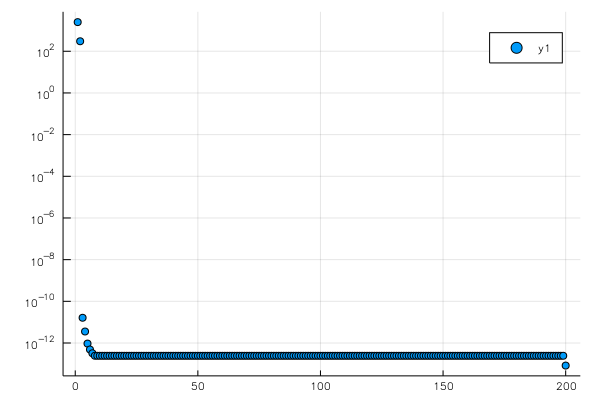
\includegraphics[width=\linewidth]{eigvalb1}
    \subcaption{Eigenvalues of $\mathcal{B}_1$}
  \end{minipage}
  \begin{minipage}[b]{0.5\linewidth}
    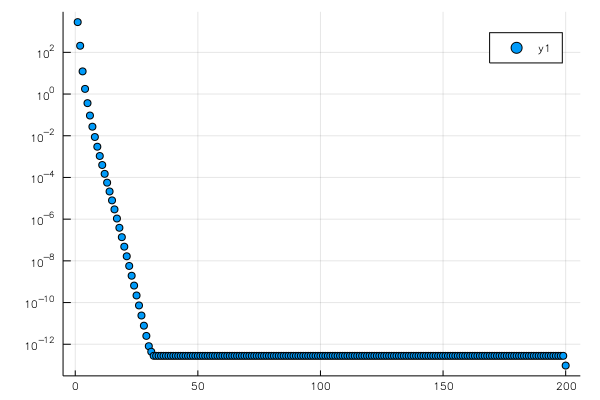
\includegraphics[width=\linewidth]{eigvalb2}
    \subcaption{Eigenvalues of $\mathcal{B}_2$}
  \end{minipage}
  \caption{Eigenvalues of 1--mode matricisation of $\mathcal{B}_1$ and $\mathcal{B}_2$}
  \label{fig:eigvals}
\end{figure}


\section{Multilinear ranks of $\mathcal{B}_1$}
\label{sec:mrb1}
\begin{quotation}
  \noindent
  Formulate a conjecture on the multilinear ranks of $\mathcal{B}_1$
  and prove it.
\end{quotation}

From the singular values as seen in
the plot (figure \ref{fig:eigvals}) of the first task, the multilinear ranks of $\mathcal{B}_1$
seem to be 2 for all matricisations, i.\,e. $\mathcal{B}_1$ has
multilinear rank $(2, 2, 2)$.

In order to show this, have a look at the structure of $\mathcal{B}_1$
and try to bring it in a form that looks like
$f_1(x)g_1(y) + f_2(x)g_2(y)$.  This is in fact a sum of two rank one
matrices expressed as functions of $x$ and $y$.  Only two variables
are used, because here we have a matrix, not a tensor.
\begin{align*}
  \mathcal{B}_1 \left(i_1, i_2, i_3 \right) &= \sin\left(\xi(i_1) + \xi(i_2) + \xi(i_3)\right) \\
                                           &= \sin\left(\xi(i_1)\right)\cos\left(\xi(i_2) + \xi(i_3)\right) +
                                               \cos\left(\xi(i_1)\right)\sin\left(\xi(i_2) + \xi(i_3)\right)\\
  &= f_1(x)g_1(y) + f_2(x)g_2(y)
\end{align*}
This is just the application of addition theorem for $\sin$.  The
result shows that the $1$--mode matricisation of $\mathcal{B}_1$ has
rank 2.  As the the $\xi(i_j)$ can be exchanged for $j$ ($\mathcal{B}_1$ is
symmetric), this result holds true for the other matricisations as
well.

Note: in fact it was proven that $\mathcal{B}_1$ has multilinear rank
$(2,2,2)$ as a function. Of course this is translates directly to the
tensor seen as multidimensional array of numbers.

\section{Matricisations of $\mathcal{B}_2$}
\label{sec:matb2}
\begin{quotation}
  \noindent
  Prove that the three different matricisations of $\mathcal{B}_2$ are
  always identical.
\end{quotation}
Here the task is to show that all three matricisations of
$\mathcal{B}_2$ are equal.

For ease of notation use a multiindex for the coloumns of
matricisation. This will show to come in very handy, in particular
when the fact that all mode sizes are equal and the tensor has order
3, i.\,e.  $\mathcal{B}_2 \in \mathbb{R}^{n \times n \times n}$ is
used.
\begin{align*}
  \mathcal{B}_2^{(1)}(i, (j, k)) &= \mathcal{B}_2 (i, j, k) \\
  \mathcal{B}_2^{(2)}(i, (j, k)) &= \mathcal{B}_2 (j, i, k) \\
  \mathcal{B}_3^{(2)}(i, (j, k)) &= \mathcal{B}_2 (j, k, i)
\end{align*}
The linear index $l$ for coloumns of the matricisation can easily be obtained by $l = j +(k-1)n$.

Now note that if the indices of $\mathcal{B}_2$ are permuted one
obtains the same number, as addition is commutative.  This inplies, if
the sum of the indices is the same also the number resulting of the
evaluation of $\mathcal{B}_2$ is the same.  So the indices
$(i, j, k)$, $(j, i, k)$, and $(j, k, i)$ all result in the same
number.  Thus the three matricisations are the identical.

\section{Adaptive Cross Approximation}
\label{sec:aca}
\begin{quotation}
  \noindent
  Develop and implement a variant of the HOSVD that uses DEIM or
  adaptive cross approximation instead of one or all three involved
  matricisations. Apply it to $\mathcal{B}_1$ and
  $\mathcal{B}_2$. What is the largest value of $n$ you can handle?
\end{quotation}

\paragraph{Motivation}
The HOSVD uses the truncated SVD to approximate the
matricisations. This is provably the best one can do in terms of
correctness for euclidean and frobenius norm.  Nevertheless other
approximation schemes, that have other advantages, can be used.  Here
the adaptive cross approximation (ACA) is used.  This does not need
the full matrix, it is possible to operate on a subset of the rows and
coloumns of the full matrix in order to obtain the approximation.

\paragraph{Adaptive Cross Approximation}
The goal of ACA is to approximate a matrix $A$ with a subset of its
own columns and rows. These subsets are denoted by $I$ and $J$,
respectively.  The approximation $\tilde{A}$ is then given by
\begin{equation*}
  \tilde{A} = A(:,J) S^{-1} A(I,:)
\end{equation*}
In this equation $S$ is $A(I,J)$.

To compute a good ACA there are several choices for the algorithm.  In
the lecture ACA with full pivoting and ACA with partial pivoting were
presented.  The algorithm chooses in every step $k$ one row and
coloumn to minimise the residual of the previous step $R_{k-1}$.  For
full pivotin the row and coloumn of the maximal element of $R_{k-1}$
is coosen.
\begin{equation*}
  (i_k, j_k) = \arg\max_{i,j} R_{k-1}(i, j)
\end{equation*}
This approach has the disadvantage of needing the full matrix
$R_{k-1}$ at every step.

The idea of not forming the full residuals explicitly but rather
compute the entries recursively as needed leads to ACA with partial
pivoting.  Here a simple line search is done for both $i$ and $j$.
\begin{align*}
  j^* &:= \arg\max_j R_{k-1})(i^*, j) \\
  i^* &:= \arg\max_i R_{k-1})(i, j^*)
\end{align*}


\paragraph{Implementation}
The algorithm presented in the lecture had to be adjusted in order to
work for the purpose of this exercise.  There are two implementations
of the ACA, one for matrices given in functional form, i.\,e. a
function taking two indices as input and returning the number at this
index, the other taking a full array as input. Both return the index
sets $I$ and $J$ for the approximation. The output matrices have to be
formed afterwards.

The algorithm for full matrices is shown in algorithm \ref{alg:aca_full}
\begin{algorithm}
  \caption{ACA for full matrices}
  \label{alg:aca_full}
  \begin{algorithmic}[1]
    \Require $A \in \mathbb{R}^{n \times m}, \eps$
    \State Set $R_0 = A: k=0: i=1$
    \State Set $I_{seen}, J_{seen} = \{\}: I^*,J^* = \{\}; \|A_1\|_F := 0$
    \Loop
      \State $i,j := find\_pivot(R_{k-1}, i, I_{seen}, J_{seen})$
      \State $I_{seen} := I_{seen} \cup \{i\}; J_{seen} = J_{seen} \cup \{j\}$
      \State $\delta_k := R_{k-1}(i,j)$
      \If{$| \delta | \leq \eps$}
        \If{$| I_{seen} | = \min (n, m) - 1$}
          \State \textbf{return} $I^*, J^*$
        \EndIf
        \State $i,j := find\_pivot(R_{k-1}, i, I_{seen}, J_{seen})$\Comment{retry one time}
        \State $\delta_k := R_{k-1}(i,j)$
        \If{$| \delta | \leq \eps$}
          \If{$| I_{seen} | = \min (n, m) - 1$}
            \State \textbf{return} $I^*, J^*$
          \EndIf
        \EndIf
      \Else
        \State $u_k := R_{k-1}(:,j); v_k := R_{k-1}(i,:)^T/\delta$
        \State $R_k := R_{k-1} - u_k v_k$
        \State $k := k+1$
        \State $I^* = I^* \cup \{i\}, J^* = J^* \cup \{j\}$
        \State $\| A_{k} \|_F^2 := \| A_{k-1} \|_F^2 + 2\sum_{j=1}^k u_k^T u_j v_j v_k^T + u_k^T u_K v_k v_k^T$
        \If{$u_k^T u_k v_k v_k^T \leq \eps \| A_{k} \|_F^2$ or $k=\min(n,m)$}
          \State \textbf{return} $I^*, J^*$
        \EndIf
      \EndIf
    \EndLoop
  \end{algorithmic}
\end{algorithm}
The function \texttt{find\_pivot} used in algorithm \ref{alg:aca_full}
is a very simple line search, see algortihm \ref{alg:pivot}. It is
iterated three times in order to get slightly better results than
using just one iteration.
\begin{algorithm}
  \caption{find\_pivot}
  \label{alg:pivot}
  \begin{algorithmic}[1]
    \Require $A \in \mathbb{R}^{n \times m}, i \in \mathbb{N}$, sets $I, J \subset \mathbb{N}$
    \For{$l = 1,2,3$}
      \State $j = \arg\max_{j \notin J} |A(i,j)|$
      \State $i = \arg\max_{i \notin I} |A(i,j)|$
    \EndFor
    \State \textbf{return} $i, j$
  \end{algorithmic}
\end{algorithm}

The ACA used for matrices given as functions is essentially
implemented the same way.  Only the updates of the residuals is more
involved.  In every step $R_k$ is recalculated from scratch.  In this
setting $R_k$ is a function returning
$(A(:,J)A(I,J)^{-1}A(I,:))_{i,j}$ for input $i, j$.  This is done by
first calculating the inverse of $A(I,J)$, then this is multiplied
with $A(i,J)$ and $A(I,j)$ from left and right, respectively.  The
advantage of this approach is, that only two small vectors and the
small matrix $S$, that is $A(I,J)^{-1}$, have to be calculated
explicitly.  Everything else is done on demand via function
evaluations.

% This update is done in algorithm \ref{alg:rk}.
% \begin{algorithm}
%   \caption{update\_rk}
%   \label{alg:rk}
%   \begin{algorithmic}
%     \Require $A: \mathbb{N}\times\mathbb{N} \rightarrow \mathbb{R}$, sets $I, J \subset \mathbb{N}$
%     \State $S := (A(I,J))^{-1}$
%     \State 


%   \end{algorithmic}
% \end{algorithm}

\end{document}
